% kompilace xelatex prezentace.tex
% dokumentace k beameru: http://ftp.cvut.cz/tex-archive/macros/latex/contrib/beamer/doc/beameruserguide.pdf

% nastavení formátu prezentace 16:9 
\documentclass[czech,aspectratio=169]{beamer}

\usepackage{polyglossia}
\setmainlanguage{czech}

% nastavení vzhledu 
% další možnosti vzhledu viz https://hartwork.org/beamer-theme-matrix/
\usetheme{Madrid}
\usecolortheme{whale}

% vzhled slajdů vnitřní téma (např. vzhled odrážek)
\useinnertheme{rectangles} %možnosti: default circles rectangles rounded inmargin
% vzhled slajdů vnější téma
\useoutertheme{default} %možnosti: default, miniframes, smoothbars, sidebar, split, shadow, tree, smoothtree, infolines

% zavedeme čvutí modou barvu
\definecolor{CVUT}{HTML}{0065BD}
% čvutí modou použijeme jako hlavní barvu prezentace
\setbeamercolor{structure}{bg=white,fg=CVUT}

% jako font prezentace nadefinujeme oficiální ČVUT písmo Technika -- pokud chcete použít, musíte si font nainstalovat nebo jej nahrát na Overleaf
% https://www.cvut.cz/logo-a-graficky-manual  -- inforek, přihlášení přes celoškolské heslo
%\usepackage{fontspec}
%\setsansfont{Technika-Kniha}

% vypneme navigační panel beamer (pro zapnutí zakomentujeme)
\beamertemplatenavigationsymbolsempty

% vygenerujeme slajdy s poznámkami -- ty si můžete vytisknout a mít je na obhajobu s sebou (pokud zapomenete slova, nebo kdyby nefungovalo promítání z nějakého důvodu)
%\setbeameroption{show notes} 

% vygeneruje slajdy s poznámky vhodné pro promítání na dvou monitorech -- na obhajobu nevyužijete
%\usepackage{pgfpages}
%\setbeameroption{show notes on second screen}

% další balíčky
\usepackage{graphicx}
\usepackage{minted}
\usepackage{hyperref}
\usepackage{tikz}
\usetikzlibrary{chains,fit,shapes}

% Údaje o prezentaci
\title[Framework for Extraction of Wikipedia Articles Content]{Framework for Extraction of Wikipedia Articles Content}
\subtitle{Diplomová práce}
\institute[FIT ČVUT v Praze]{Fakulta informačních technologií \\ České vysoké učení technické v Praze}
\author[Oleksandr Husiev]{Oleksandr Husiev \\ Vedoucí práce: Ing. Milan Doj{\v c}inovski, Ph. D.}
\date{07. 12. 2021}
\titlegraphic{
\includegraphics[width=.1\textwidth]{logo-cvut}}


\begin{document}
    \begin{frame}
        \titlepage
    \end{frame}
    
    \begin{frame}
        \tableofcontents
    \end{frame}
  
    \section{Thesis goals}
    
    \begin{frame}{Thesis goals}
    	
    	DBpedia is a crowd-sourced community effort that aims at extraction of information from Wikipedia. Vast amounts of information are not yet extracted from the Wikipedia texts. The main goal of the thesis is to develop a framework for extraction of Wikipedia articles content, structure and annotations which can be further split into those subgoals:
    	
        \begin{itemize}
            \item Accept and process input data in the form of Wikipedia XML dumps
            \item Extract Wikipedia context, page structure, and links.
            \item Provide outputs for context, links and page structure in the form of N-Triples.
            \item Implement language extensibility.
            \item Provide a user interface to interact with the framework.
        \end{itemize}
    \end{frame}
    
    \section{Motivation}
    \begin{frame}{Motivation}
        \begin{itemize}
            \item Motivace 1
            \item Motivace 2
            \item Motivace 3
            \item Motivace 4
            \item Motivace 5
        \end{itemize}
    \end{frame}
  
    \section{Sekce 1}
    \begin{frame}{Sekce 1}
        \begin{itemize}
            \item item 1
            \item item 2
            \item item 3
            \item item 4
        \end{itemize}
    \end{frame}
    
    \begin{frame}{Snimek s obrazkem}
        \begin{center}
            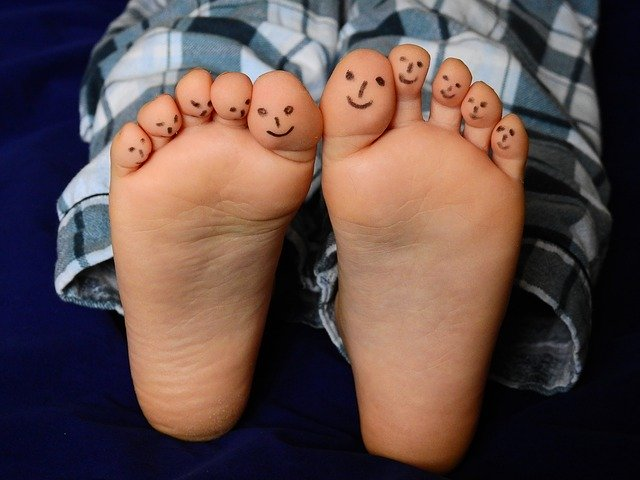
\includegraphics[width=0.6\paperwidth]{pic01.jpg}
        \end{center}
    \end{frame}
    
    \section{Analýza}
    \begin{frame}{Analýza}
        \begin{itemize}
            \item Analyza 1
            \item Analyza 2
            \item Analyza 3
            \item Analyza 4
            \item Analyza 5
            \item Analyza 6
        \end{itemize}
    \end{frame}
    
    \section{Realizace 1}
    \begin{frame}{Realizace 1}{podtitulek realizace 1}
        \begin{itemize}
            \item Dokonceno 1
            \item Dokonceno 2
            \item Dokonceno 3
            \item Dokonceno 4
        \end{itemize}
    \end{frame}
    
    \begin{frame}{Realizace 2}{podtitulek realizace 2}
        \begin{itemize}
            \item Dokonceno 1
            \item Dokonceno 2
        \end{itemize}
    \end{frame}
    
    \section{Design neceho}
    \begin{frame}{Design neceho}{podtitulek design neceho}
        \begin{itemize}
            \item Pozadavek na design 1
            \item Pozadavek na design 2
            \item Pozadavek na design 3
            \item Pozadavek na design 4
        \end{itemize}
    \end{frame}
    
    \begin{frame}{Design neceho}{design ceho}
        \begin{center}
            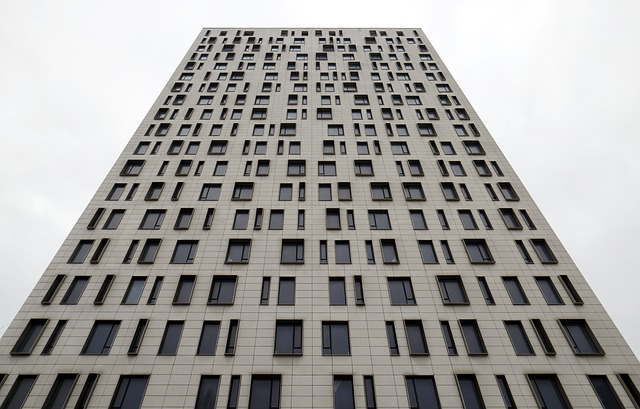
\includegraphics[width=0.6\paperwidth]{pic02.jpg}
        \end{center}
    \end{frame}
    
    \begin{frame}{Design neceho}{design ceho}
        \begin{center}
            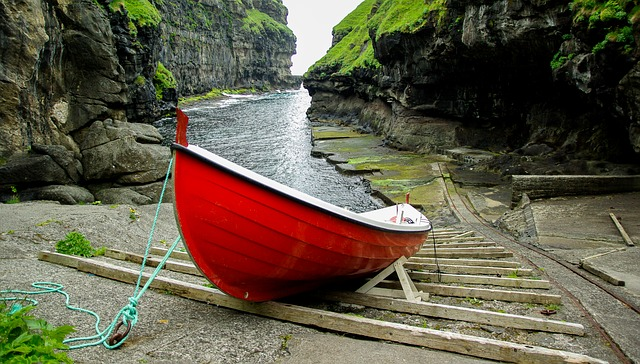
\includegraphics[width=0.7\paperwidth]{pic03.jpg}
        \end{center}
    \end{frame}
    
    \begin{frame}{Design neceho}{design ceho}
        \begin{center}
            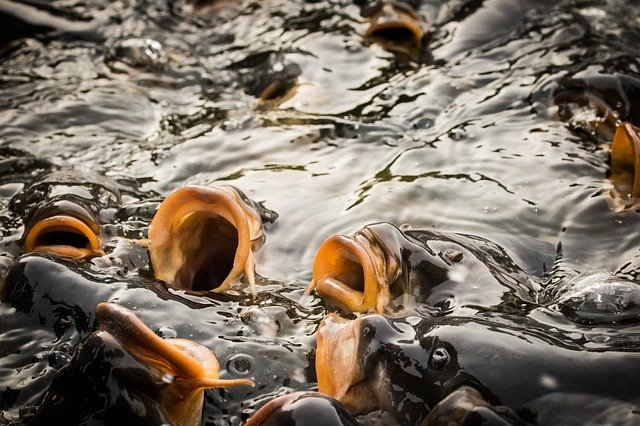
\includegraphics[width=0.6\paperwidth]{pic04.jpg}
        \end{center}
    \end{frame}
    
    \section{Testování}
    \begin{frame}{Testování}
        \begin{itemize}
            \item Testování neceho 1
            \item Testování neceho 2
            \item Testování neceho 3
            \item Testování neceho 4
        \end{itemize}
    \end{frame}

    \begin{frame}{Shrnutí}
        \begin{itemize}
            \item shrnuti 1
            \item shrnuti 2
            \item shrnuti 3
            \item shrnuti 4
            \item shrnuti 5
            \item shrnuti 6
        \end{itemize}
    
    \end{frame}
    
    \begin{frame}{Konec}
        \center Děkuji za pozornost!
    \end{frame}

    \begin{frame}[noframenumbering]{Otázky oponenta}
        Otázka první: Proč?
    
        \vfill
    
        Odpověď: Prostě proto.
    \end{frame}
    
    \begin{frame}[noframenumbering]{Otázky oponenta}
        Otázka druhá: Proč?
    
        \vfill
    
        Odpověď: Prostě proto.
    \end{frame}

\end{document}